\section{Funcions contínues}

\textbf{Definició:} Una funció $f(x)$ és \textbf{contínua} en el punt $x = a$ si es verifiquen les dues condicions següents:

\begin{itemize}
\item Existeix $f(a)$; és a dir, $a$ pertany al domini de la funció.
\item Existeixen els límits laterals de $f(x)$ en el punt $a$ i coincideixen amb $f(a)$:
\end{itemize}

\begin{equation}
\lim_{x\to a^-} f(x) = \lim_{x\to a^+} f(x) = f(a)
\end{equation}

Una funció és contínua en un interval si ho és en tots i cadascun dels punts de l'interval. Podem afirmar també que totes les funcions polinòmiques són funcions contínues.

La figura il\textperiodcentered{}lustra la diferència entre una funció contínua i una de no contínua en el punt $a$:

\begin{figure}[!htbp]
\centering
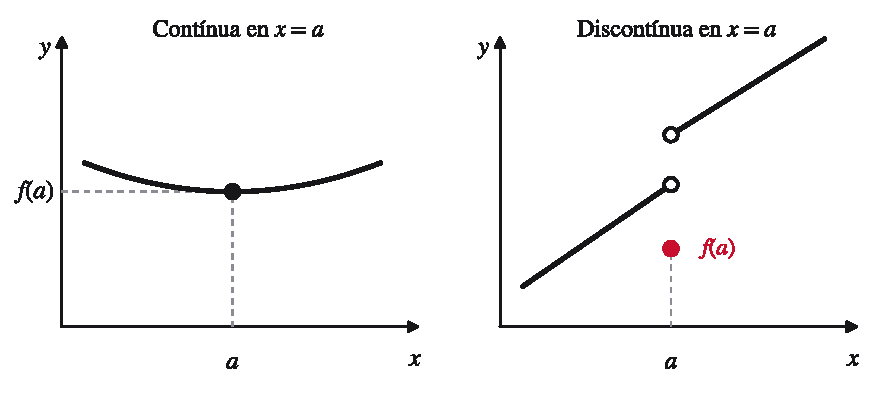
\includegraphics[width=424pt]{fig/m02_f03.pdf}
\caption{A l'esquerra, funció contínua en $x = a$: el límit coincideix amb $f(a)$. A la dreta, funció discontínua en $x = a$: els límits laterals no coincideixen amb el valor de la funció.}
\end{figure}

\section{Propietats de les funcions contínues}

\subsection{Teorema dels valors intermedis}

\textbf{Propietat (Teorema dels valors intermedis):} Sigui $f(x)$ una funció contínua en un interval tancat $[a, b]$ i $k$ un nombre tal que $f(a) \le k \le f(b)$. Aleshores, existeix almenys un punt $c \in [a, b]$ tal que $f(c) = k$.

\begin{figure}[!htbp]
\centering
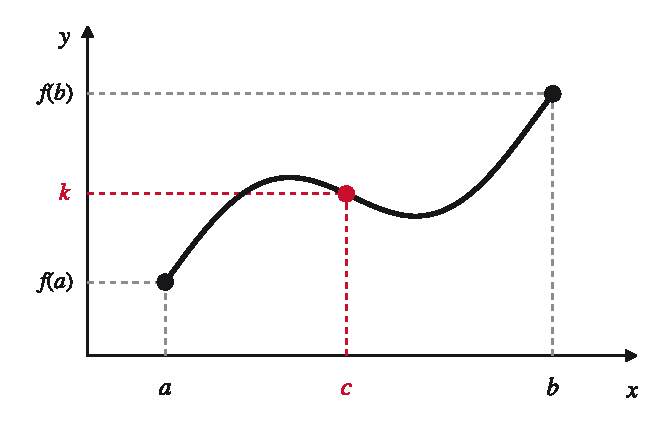
\includegraphics[width=319pt]{fig/m02_f04.pdf}
\caption{Il\textperiodcentered{}lustració del Teorema dels valors intermedis: per a tot $k$ entre $f(a)$ i $f(b)$, existeix $c \in [a, b]$ tal que $f(c) = k$.}
\end{figure}

\subsection{Teorema de Bolzano}

\textbf{Propietat (Teorema de Bolzano):} Sigui $f(x)$ una funció contínua en un interval tancat $[a, b]$ tal que $f(a)\cdot f(b) < 0$ (és a dir, $f(a)$ i $f(b)$ tenen signe diferent). Aleshores, existeix almenys un punt $c \in (a, b)$ tal que $f(c) = 0$.

\begin{figure}[!htbp]
\centering
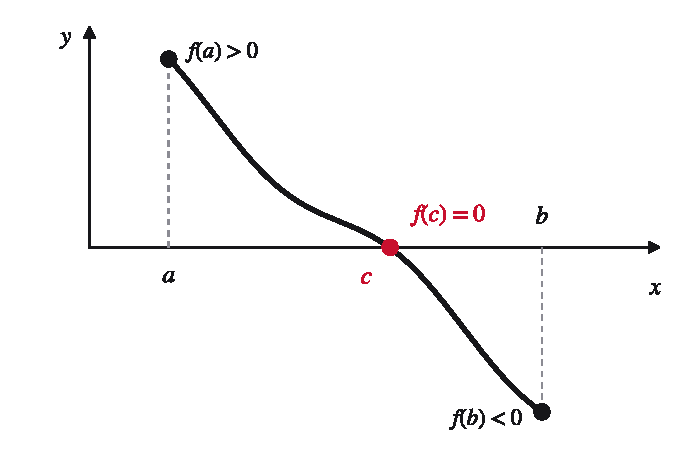
\includegraphics[width=330pt]{fig/m02_f05.pdf}
\caption{Teorema de Bolzano: $f(a) > 0$, $f(b) < 0$ i $f$ contínua en $[a, b] \Rightarrow \exists\, c \in (a, b)$ tal que $f(c) = 0$.}
\end{figure}

\section{Màxims i mínims absoluts d'una funció en un interval}

Considerem una funció $f(x)$ contínua en un interval tancat $[a, b]$. Aleshores:

\begin{itemize}
\item Existeix almenys un punt $c \in [a, b]$ en què la funció assoleix el seu \textbf{valor màxim absolut}, és a dir, $f(c) \ge f(x)$ per a tot $x \in [a, b]$.
\item Existeix almenys un punt $d \in [a, b]$ en què la funció assoleix el seu \textbf{valor mínim absolut}, és a dir, $f(d) \le f(x)$ per a tot $x \in [a, b]$.
\end{itemize}

\begin{figure}[!htbp]
\centering
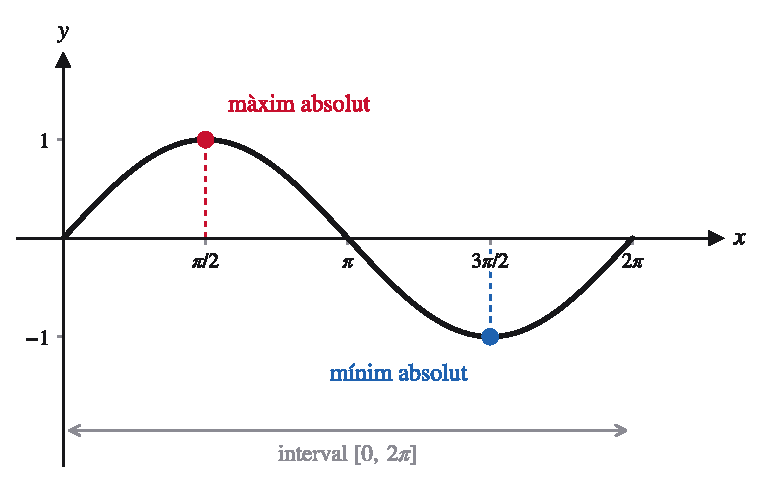
\includegraphics[width=367pt]{fig/m02_f06.pdf}
\caption{Màxim i mínim absoluts de $f(x) = \sin x$ en l'interval $[0, 2\pi]$.}
\end{figure}

\section{Funcions derivables}

\textbf{Definició:} Una funció contínua $f(x)$ és \textbf{derivable} en un punt $x = x_0$ si existeix $f'(x_0)$:

\begin{equation}
f'(x_0) = \lim_{h\to 0} \frac{f(x_0 + h) - f(x_0)}{h}
\end{equation}

Cal tenir present la relació entre continuïtat i derivabilitat:

\begin{itemize}
\item Si una funció és discontínua en un punt, no és derivable en aquell punt.
\item Una funció derivable en un punt és necessàriament contínua en aquell punt.
\end{itemize}

\subsection{Tipus de discontinuïtats}

Si $f(x)$ no és derivable en $x_0$, el límit $\displaystyle\lim_{h\to 0}\frac{f(x_0+h)-f(x_0)}{h}$ no existeix. Podem distingir tres casos:

\begin{itemize}
\item \textbf{Discontinuïtat evitable:} no existeix $f(x_0)$ i, per tant, tampoc el límit de la diferència.
\item \textbf{Discontinuïtat de salt:} el límit no existeix perquè els límits laterals a dreta i esquerra de $x_0$ no coincideixen.
\item \textbf{Discontinuïtat asimptòtica:} el límit no és numèric (un dels dos límits laterals o tots dos tendeixen a l'infinit).
\end{itemize}

La figura mostra els cinc casos possibles de no-derivabilitat o discontinuïtat en un punt $a$:

\begin{figure}[!htbp]
\centering
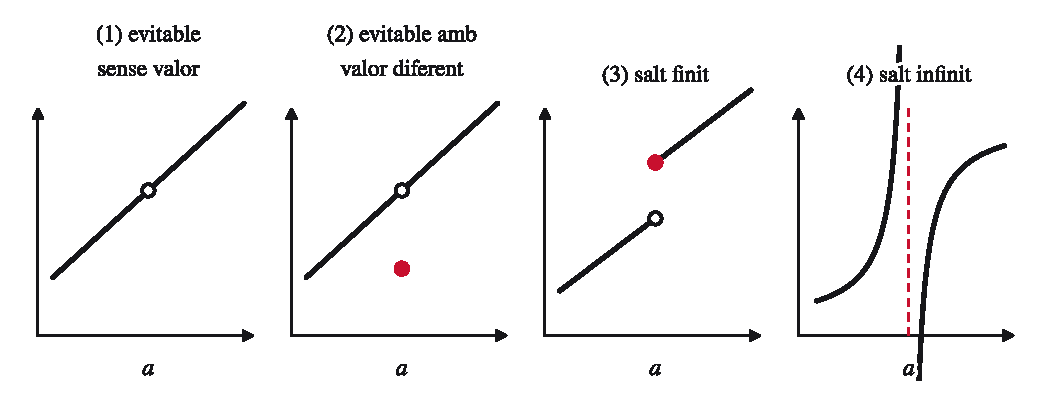
\includegraphics[width=440pt]{fig/m02_f07.pdf}
\caption{Tipus de discontinuïtats en un punt $a$: evitable sense valor (1), evitable amb valor diferent (2), salt finit (3) i salt infinit o asimptòtica (4).}
\end{figure}

\section{Propietats de les funcions derivables}

\subsection{Teorema de Rolle}

\textbf{Propietat (Teorema de Rolle):} Si $f(x)$ és contínua en $[a, b]$, derivable en $(a, b)$ i $f(a) = f(b)$, aleshores existeix almenys un punt $c \in (a, b)$ tal que $f'(c) = 0$.

\begin{figure}[!htbp]
\centering
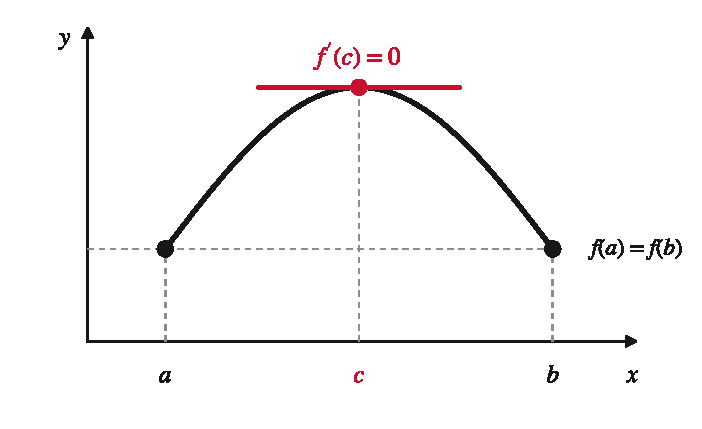
\includegraphics[width=337pt]{fig/m02_f08.pdf}
\caption{Teorema de Rolle: si $f(a) = f(b)$, existeix $c \in (a, b)$ on la tangent és horitzontal, és a dir, $f'(c) = 0$.}
\end{figure}

\subsection{Teorema del valor mitjà (Lagrange)}

\textbf{Propietat (Teorema del valor mitjà):} Si $f(x)$ és contínua en $[a, b]$ i derivable en $(a, b)$, existeix almenys un punt $c \in (a, b)$ tal que

\begin{equation}
f'(c) = \frac{f(b) - f(a)}{b - a}
\end{equation}

Geomètricament, el teorema afirma que existeix un punt $c$ on la tangent a la corba és paral\textperiodcentered{}lela a la secant que uneix $(a, f(a))$ i $(b, f(b))$.

\begin{figure}[!htbp]
\centering
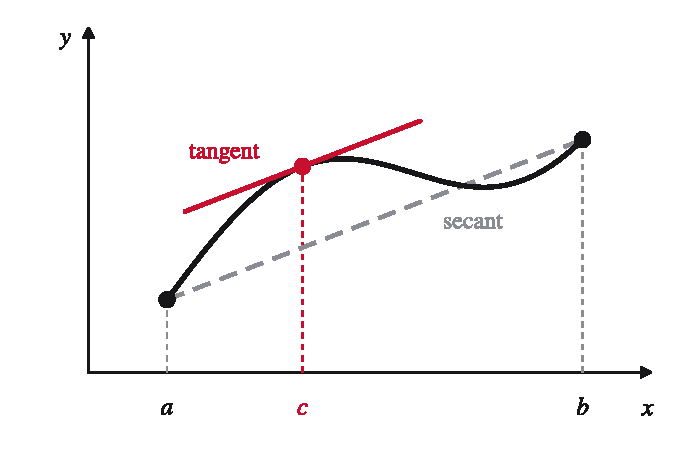
\includegraphics[width=330pt]{fig/m02_f09.pdf}
\caption{Teorema del valor mitjà: en algun punt $c \in (a, b)$, la tangent a la corba és paral\textperiodcentered{}lela a la recta secant que uneix $(a, f(a))$ i $(b, f(b))$.}
\end{figure}

\subsection{Teorema de Cauchy}

\textbf{Propietat (Teorema de Cauchy):} Si $f(x)$ i $g(x)$ són dues funcions contínues en $[a, b]$ i derivables en $(a, b)$, aleshores existeix un punt $c \in (a, b)$ tal que

\begin{equation}
\frac{f(b) - f(a)}{g(b) - g(a)} = \frac{f'(c)}{g'(c)}
\end{equation}

El teorema de Cauchy és una generalització del teorema del valor mitjà: si $g(x) = x$, aleshores $g'(c) = 1$ i es recupera exactament el resultat de Lagrange.

\section{La segona derivada}

La segona derivada d'una funció s'obté derivant la funció derivada:

\begin{equation*}
f''(x) = [f'(x)]'
\end{equation*}

La segona derivada permet caracteritzar els extrems relatius i la concavitat de la funció.

\subsection{Màxims i mínims relatius}

\begin{itemize}
\item Si $f'(x_1) = 0$ i $f''(x_1) < 0$, en $x = x_1$ hi ha un \textbf{màxim relatiu} de $f(x)$.
\item Si $f'(x_2) = 0$ i $f''(x_2) > 0$, en $x = x_2$ hi ha un \textbf{mínim relatiu} de $f(x)$.
\end{itemize}

\subsection{Concavitat d'una funció}

\begin{itemize}
\item $f(x)$ és \textbf{convexa} (còncava cap avall, $\cap$) en un interval si $f''(x) < 0$ per a tot $x$ de l'interval.
\item $f(x)$ és \textbf{còncava} (còncava cap amunt, $\cup$) en un interval si $f''(x) > 0$ per a tot $x$ de l'interval.
\end{itemize}

\subsection{Punt d'inflexió}

Si $f''(x)$ és contínua en l'interval considerat i passa de positiva a negativa (o a l'inrevés), necessàriament existirà un punt en què $f''(x) = 0$. En aquest punt canvia la concavitat de la gràfica i s'anomena \textbf{punt d'inflexió}.

\begin{figure}[!htbp]
\centering
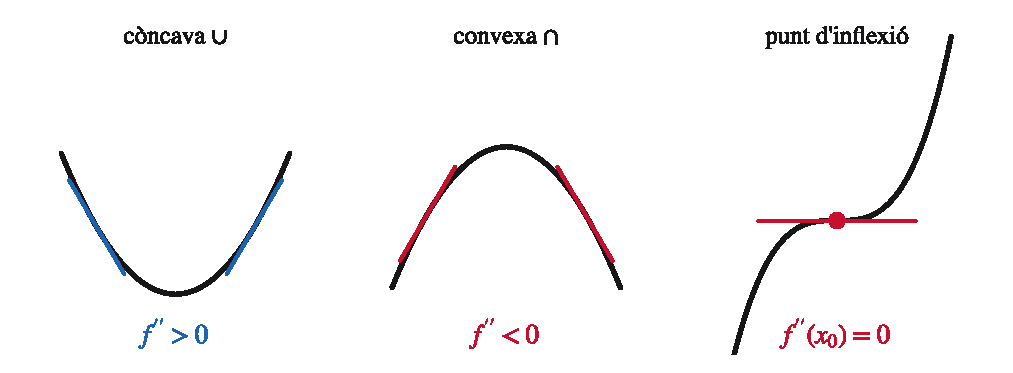
\includegraphics[width=440pt]{fig/m02_f10.pdf}
\caption{Concavitat: còncava cap amunt ($\cup$, $f'' > 0$), convexa cap avall ($\cap$, $f'' < 0$) i punt d'inflexió on canvia la concavitat ($f''(x_0) = 0$).}
\end{figure}

\section{Càlcul de límits i la derivada. Regla de l'Hôpital}

\textbf{Propietat (Regla de l'Hôpital):} Siguin $f$ i $g$ funcions derivables en un entorn de $x_0$, amb $g'(x) \neq 0$. Si el quocient $f(x)/g(x)$ presenta una indeterminació del tipus $0/0$ o $\infty/\infty$ en $x_0$, aleshores

\begin{equation}
\lim_{x\to x_0} \frac{f(x)}{g(x)} = \lim_{x\to x_0} \frac{f'(x)}{g'(x)}
\end{equation}

sempre que el límit del costat dret existeixi.

La regla s'aplica en els casos d'indeterminació del tipus $\dfrac{0}{0}$ i $\dfrac{\infty}{\infty}$, i pot aplicar-se repetidament si el quocient de les derivades continua sent indeterminat.

En els càlculs de límits, les expressions indeterminades més habituals són:

\begin{equation*}
\frac{0}{0},\quad \frac{\infty}{\infty},\quad \infty\cdot 0,\quad 1^\infty,\quad \infty^0,\quad 0^0,\quad \infty-\infty
\end{equation*}

\emph{Observació:} les indeterminacions del tipus $\infty\cdot 0$, $1^\infty$, $\infty^0$ i $0^0$ es redueixen prèviament a una forma $0/0$ o $\infty/\infty$ (per exemple, mitjançant logaritmes o inversions) per poder aplicar la regla de l'Hôpital.

\section{Complement: càlcul de límits}

\subsection{Límits laterals i límits a l'infinit}

El límit $\displaystyle\lim_{x\to a} f(x) = L$ existeix si i només si els \textbf{límits laterals} coincideixen:

\begin{equation*}
\lim_{x\to a^-} f(x) = \lim_{x\to a^+} f(x) = L
\end{equation*}

Si el límit és $\pm\infty$, hi ha una \textbf{asímptota vertical} $x = a$. Si $\displaystyle\lim_{x\to\pm\infty} f(x) = b$, hi ha una \textbf{asímptota horitzontal} $y = b$.

Per a $x\to+\infty$, les funcions elementals es poden ordenar per ordre de creixement:

\begin{equation*}
\ln x \;\ll\; x^n \;\ll\; a^x \;\;(a>1)
\end{equation*}

És a dir, una exponencial supera qualsevol potència, i una potència supera qualsevol logaritme. Això resol molts límits $\infty/\infty$ de cop d'ull.

\subsection{Les indeterminacions i com resoldre-les}

\begin{table}[!htbp]
\centering
\renewcommand{\arraystretch}{1.75}
\begin{tabularx}{\textwidth}{l>{\raggedright\arraybackslash}X}
\toprule
Indeterminació & Com tractar-la \\
\midrule
$\displaystyle \dfrac{0}{0}$ & Factoritzar i simplificar (polinomis); multiplicar pel \textbf{conjugat} (arrels); regla de l'Hôpital \\
$\displaystyle \dfrac{\infty}{\infty}$ & Dividir per la \textbf{potència més alta} de $x$ (només comparar graus); comparar ordres de creixement; Hôpital \\
$\infty - \infty$ & Fraccions: denominador comú. Arrels: multiplicar i dividir pel \textbf{conjugat} \\
$0\cdot\infty$ & Convertir en quocient $\displaystyle \frac{0}{0}$ o $\displaystyle \frac{\infty}{\infty}$ i aplicar Hôpital \\
$1^{\infty}$ & Fórmula del nombre $e$ (vegeu a sota) \\
$0^0,\ \infty^0$ & Prendre logaritmes: $\ln L = \lim g\cdot\ln f$ \\
\bottomrule
\end{tabularx}
\end{table}

\textbf{Límits notables} (per a $x\to 0$):

\begin{equation*}
\lim_{x\to0}\frac{\sin x}{x}=1,\qquad \lim_{x\to0}\frac{1-\cos x}{x^2}=\frac12,\qquad \lim_{x\to0}\frac{e^x-1}{x}=1,\qquad \lim_{x\to0}\frac{\ln(1+x)}{x}=1
\end{equation*}

\textbf{Indeterminació $1^\infty$.} Si $\displaystyle\lim_{x\to a} f(x)=1$ i $\displaystyle\lim_{x\to a} g(x)=\pm\infty$, aleshores

\begin{equation*}
\lim_{x\to a} f(x)^{g(x)} = e^{\,\lim_{x\to a} g(x)\,\bigl(f(x)-1\bigr)}
\end{equation*}

\subsection{Exemples resolts}

\textbf{a)} $\displaystyle\lim_{x\to2}\frac{x^2-4}{x-2}\;\;\left(\tfrac00\right)$: es factoritza $x^2-4=(x-2)(x+2)$ i es simplifica:

\begin{equation*}
\lim_{x\to2}(x+2)=4
\end{equation*}

\textbf{b)} $\displaystyle\lim_{x\to0}\frac{\sqrt{x+4}-2}{x}\;\;\left(\tfrac00\right)$: es multiplica pel conjugat.

\begin{equation*}
\frac{(\sqrt{x+4}-2)(\sqrt{x+4}+2)}{x(\sqrt{x+4}+2)}=\frac{x}{x(\sqrt{x+4}+2)}=\frac{1}{\sqrt{x+4}+2}\;\longrightarrow\;\frac14
\end{equation*}

\textbf{c)} $\displaystyle\lim_{x\to+\infty}\frac{3x^2-x+1}{5x^2+2}\;\;\left(\tfrac\infty\infty\right)$: mateix grau, el límit és el quocient dels coeficients dominants: $\dfrac35$.

\emph{Regla pràctica per a quocients de polinomis en $\pm\infty$:} grau del numerador $<$ grau del denominador $\Rightarrow 0$; iguals $\Rightarrow$ quocient de coeficients; numerador de grau superior $\Rightarrow\pm\infty$.

\textbf{d)} $\displaystyle\lim_{x\to+\infty}\left(\sqrt{x^2+x}-x\right)\;\;(\infty-\infty)$:

\begin{equation*}
\frac{(\sqrt{x^2+x}-x)(\sqrt{x^2+x}+x)}{\sqrt{x^2+x}+x}=\frac{x}{\sqrt{x^2+x}+x}=\frac{1}{\sqrt{1+\frac1x}+1}\;\longrightarrow\;\frac12
\end{equation*}

\textbf{e)} $\displaystyle\lim_{x\to+\infty}\left(1+\frac2x\right)^{x}\;\;(1^\infty)$:

\begin{equation*}
e^{\lim x\left(1+\frac2x-1\right)}=e^{\lim x\cdot\frac2x}=e^2
\end{equation*}

\textbf{f)} Límits laterals amb asímptota vertical: $\displaystyle\lim_{x\to3^\pm}\frac{2x+1}{x-3}$. El numerador val $7>0$ prop de $x=3$, i el denominador és petit: positiu si $x\to3^+$ i negatiu si $x\to3^-$. Per tant

\begin{equation*}
\lim_{x\to3^+}\frac{2x+1}{x-3}=+\infty,\qquad \lim_{x\to3^-}\frac{2x+1}{x-3}=-\infty
\end{equation*}

A més, $\displaystyle\lim_{x\to\pm\infty}\frac{2x+1}{x-3}=2$: asímptota horitzontal $y=2$.

\begin{figure}[!htbp]
\centering
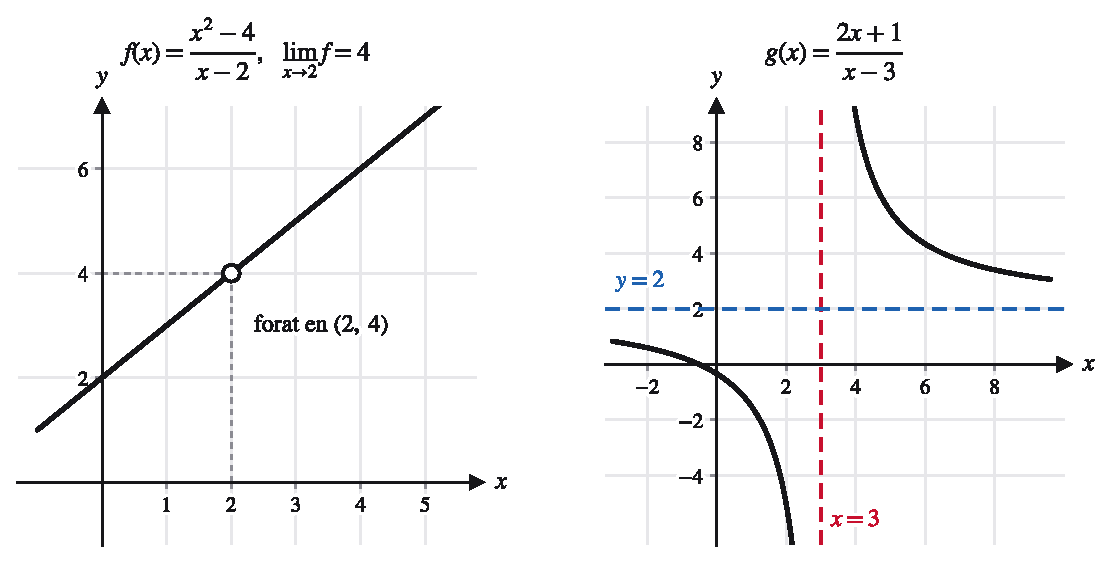
\includegraphics[width=440pt]{fig/m02_f29.pdf}
\caption{A l'esquerra, $f(x)=\dfrac{x^2-4}{x-2}$ coincideix amb $y=x+2$ excepte en $x=2$, on hi ha un forat: el límit val $4$ tot i que $f(2)$ no existeix. A la dreta, $g(x)=\dfrac{2x+1}{x-3}$ amb asímptota vertical $x=3$ i horitzontal $y=2$.}
\end{figure}

\section{Complement: funcions definides a trossos}

Una funció definida a trossos pot ser contínua i derivable en els punts on canvia l'expressió només si es compleixen unes condicions. Per a una funció

\begin{equation*}
f(x)=\begin{cases} f_1(x) & x\le a\\ f_2(x) & x>a\end{cases}
\end{equation*}

\textbf{Propietat (Continuïtat i derivabilitat en el punt de canvi):} 

\begin{itemize}
\item \textbf{Contínua en $x=a$} $\iff$ $f_1(a)=\displaystyle\lim_{x\to a^+}f_2(x)=f_2(a)$ (els dos trossos \emph{es toquen}).
\item \textbf{Derivable en $x=a$} $\iff$ és contínua \textbf{i} $f_1'(a)=f_2'(a)$ (els dos trossos \emph{s'enganxen sense angle}).
\end{itemize}

\emph{Atenció:} abans de comparar derivades cal assegurar la continuïtat. Una funció derivable sempre és contínua, però no al revés (per exemple, $f(x)=|x|$ és contínua en $0$ però no derivable: les derivades laterals valen $-1$ i $1$).

\subsection{Exemple --- Trobar paràmetres}

Determineu $a$ i $b$ perquè sigui derivable en $x=1$:

\begin{equation*}
f(x)=\begin{cases} ax^2+1 & x\le 1\\ bx-1 & x>1\end{cases}
\end{equation*}

\begin{enumerate}
\item \textbf{Continuïtat en $x=1$:} $a\cdot1^2+1=b\cdot1-1 \;\Rightarrow\; a+1=b-1 \;\Rightarrow\; b=a+2$.
\item \textbf{Derivades:} $f_1'(x)=2ax$ i $f_2'(x)=b$. En $x=1$: $2a=b$.
\item \textbf{Sistema:} $b=a+2$ i $b=2a \Rightarrow 2a=a+2 \Rightarrow a=2$, $b=4$.
\end{enumerate}

Comprovació: $f(1)=2+1=3$ pels dos costats, i les dues derivades valen $4$.

\begin{figure}[!htbp]
\centering
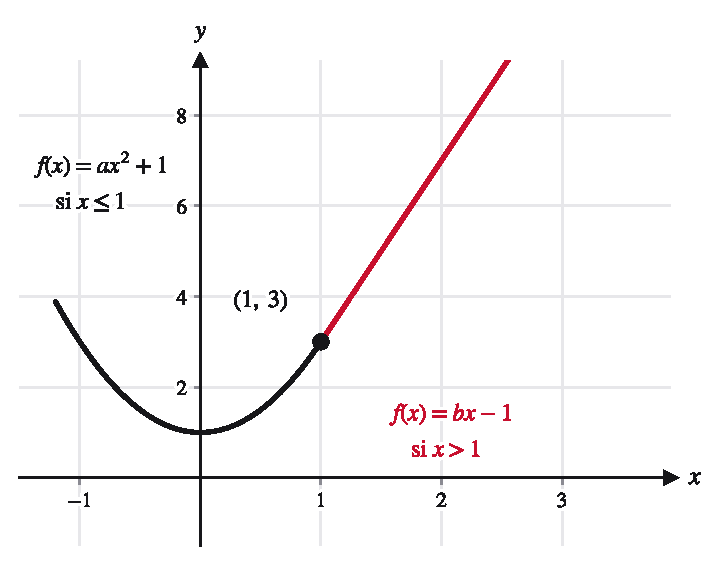
\includegraphics[width=345pt]{fig/m02_f30.pdf}
\caption{La funció a trossos amb $a=2$ i $b=4$ és contínua i derivable en $x=1$: la paràbola i la recta se uneixen en $(1, 3)$ amb el mateix pendent.}
\end{figure}

\section{Complement: demostracions dels teoremes}

Aquest apartat recull les demostracions dels teoremes d'aquest tema, perquè entenguis \textbf{d'on surten} i com s'encadenen. A la PAU normalment només cal \emph{saber aplicar-los} (comprovant les hipòtesis), però a vegades demanen explicar-ne una.

\emph{Ordre lògic:} Bolzano i Weierstrass (continuïtat) $\rightarrow$ lema de Fermat $\rightarrow$ Rolle $\rightarrow$ Lagrange $\rightarrow$ Cauchy.

\subsection{Teorema de Bolzano}

\textbf{Teorema:} si $f$ és contínua en $[a,b]$ i $f(a)\cdot f(b)<0$, existeix $c\in(a,b)$ amb $f(c)=0$.

\emph{Demostració.} Suposem $f(a)<0<f(b)$ (l'altre cas s'obté aplicant-ho a $-f$). Considerem el conjunt

\begin{equation*}
S=\{x\in[a,b]\;:\;f(x)<0\}
\end{equation*}

És no buit ($a\in S$) i està fitat superiorment per $b$; sigui $c=\sup S$. Provem que $f(c)=0$ descartant les altres dues possibilitats:

\begin{itemize}
\item \textbf{Si $f(c)<0$:} llavors $c\neq b$ (perquè $f(b)>0$). Per continuïtat, $f<0$ en un entorn de $c$, de manera que hi ha punts de $S$ més grans que $c$. Contradicció amb que $c$ és el suprem.
\item \textbf{Si $f(c)>0$:} llavors $c\neq a$. Per continuïtat, $f>0$ en un interval $(c-\delta,c]$, de manera que cap punt d'aquest interval és de $S$ i el suprem seria com a molt $c-\delta$. Contradicció.
\end{itemize}

Per tant $f(c)=0$, i com que $f(a)\neq0\neq f(b)$, $c\in(a,b)$. $\blacksquare$

\subsection{Teorema de Weierstrass (esquema)}

\textbf{Teorema:} si $f$ és contínua en $[a,b]$, existeixen $m,M$ (mínim i màxim absoluts) tals que $m\le f(x)\le M$ i $f$ pren aquests valors.

\emph{Esquema de la demostració.} \textbf{(1) $f$ està fitada.} Si no ho estigués, hi hauria una successió $x_n\in[a,b]$ amb $|f(x_n)|>n$. Com que $[a,b]$ és tancat i fitat, té una subsuccessió convergent $x_{n_k}\to x_0\in[a,b]$; per continuïtat $f(x_{n_k})\to f(x_0)$, que és un nombre finit: contradicció.

\textbf{(2) El suprem s'assoleix.} Sigui $M=\sup f$. Hi ha $x_n$ amb $f(x_n)\to M$; agafant una subsuccessió $x_{n_k}\to c\in[a,b]$, per continuïtat $f(c)=M$. Igual amb el mínim. $\blacksquare$

\subsection{Lema de Fermat}

\textbf{Lema:} si $f$ és derivable en $c$ i té un extrem relatiu en $c$ (interior a l'interval), llavors $f'(c)=0$.

\emph{Demostració.} Suposem un màxim: $f(x)\le f(c)$ prop de $c$.

\begin{itemize}
\item Per $x>c$: $\dfrac{f(x)-f(c)}{x-c}\le0$, i passant al límit, $f'(c)\le0$.
\item Per $x<c$: $\dfrac{f(x)-f(c)}{x-c}\ge0$, i passant al límit, $f'(c)\ge0$.
\end{itemize}

Com que $f'(c)$ existeix, els dos límits coincideixen: $f'(c)=0$. $\blacksquare$

\subsection{Teorema de Rolle}

\emph{Demostració.} Per Weierstrass, $f$ té màxim $M$ i mínim $m$ en $[a,b]$.

\begin{itemize}
\item \textbf{Si $M=m$}, $f$ és constant i $f'(x)=0$ en qualsevol punt de $(a,b)$.
\item \textbf{Si $M\neq m$}, com que $f(a)=f(b)$, almenys un dels dos valors (màxim o mínim) s'assoleix en un punt $c$ \textbf{interior}. Pel lema de Fermat, $f'(c)=0$. $\blacksquare$
\end{itemize}

\subsection{Teorema del valor mitjà (Lagrange)}

\emph{Demostració.} Restem de $f$ la recta secant que uneix els extrems:

\begin{equation*}
g(x)=f(x)-f(a)-\frac{f(b)-f(a)}{b-a}\,(x-a)
\end{equation*}

$g$ és contínua en $[a,b]$, derivable en $(a,b)$ i $g(a)=0=g(b)$. Per Rolle, existeix $c$ amb $g'(c)=0$, és a dir,

\begin{equation*}
f'(c)-\frac{f(b)-f(a)}{b-a}=0\;\Longrightarrow\;f'(c)=\frac{f(b)-f(a)}{b-a}.\ \blacksquare
\end{equation*}

\textbf{Conseqüència (la més usada).} Si $f'(x)>0$ en un interval, $f$ és creixent: per a $x_1<x_2$, $f(x_2)-f(x_1)=f'(c)(x_2-x_1)>0$. Igualment, si $f'(x)=0$ en tot l'interval, $f$ és constant.

\subsection{Teorema de Cauchy}

\textbf{Teorema:} si $f,g$ són contínues en $[a,b]$ i derivables en $(a,b)$, existeix $c$ amb $f'(c)\,\bigl(g(b)-g(a)\bigr)=g'(c)\,\bigl(f(b)-f(a)\bigr)$.

\emph{Demostració.} Definim $h(x)=f(x)\bigl(g(b)-g(a)\bigr)-g(x)\bigl(f(b)-f(a)\bigr)$. Es comprova que $h(a)=f(a)g(b)-g(a)f(b)=h(b)$. Per Rolle, $h'(c)=0$ per a algun $c$, que és exactament la igualtat enunciada. $\blacksquare$

\emph{Aquest teorema és la base de la regla de l'Hôpital.}

\subsection{Exemple d'aplicació d'una demostració}

\textbf{Demostra que $x^3+x-1=0$ té una única arrel real.}

\begin{itemize}
\item \emph{Existència:} $f(x)=x^3+x-1$ és contínua, $f(0)=-1<0$ i $f(1)=1>0$; per \textbf{Bolzano} hi ha una arrel a $(0,1)$.
\item \emph{Unicitat:} si hi hagués dues arrels $a<b$, com que $f(a)=f(b)=0$, per \textbf{Rolle} existiria $c$ amb $f'(c)=0$. Però $f'(x)=3x^2+1>0$ sempre: contradicció. Per tant, l'arrel és única.
\end{itemize}

\section{Complement: derivabilitat i continuïtat}

\textbf{Teorema:} Si una funció $f$ és derivable en $x=a$, aleshores és contínua en $x=a$.

\emph{Demostració.} Per a $x\neq a$ escrivim $f(x)-f(a)=\dfrac{f(x)-f(a)}{x-a}\,(x-a)$. Prenent el límit quan $x\to a$,

\begin{equation*}
\lim_{x\to a}\bigl[f(x)-f(a)\bigr]=f'(a)\cdot0=0\ \Longrightarrow\ \lim_{x\to a}f(x)=f(a).\ \blacksquare
\end{equation*}

El recíproc és fals: $f(x)=|x|$ és contínua en $x=0$ però no és derivable. Per tant, ``derivable $\Rightarrow$ contínua'', però ``contínua $\not\Rightarrow$ derivable''.

\section{Complement: aplicació dels teoremes en problemes}

Els teoremes d'aquest tema se solen aplicar per demostrar l'existència o la unicitat de solucions d'una equació.

\emph{Exemple 1 (Bolzano):} Demostrem que $x^3+x-1=0$ té alguna solució a $(0,1)$. La funció $f(x)=x^3+x-1$ és contínua a $[0,1]$, amb $f(0)=-1<0$ i $f(1)=1>0$. Pel teorema de Bolzano, existeix $c\in(0,1)$ amb $f(c)=0$.

\emph{Exemple 2 (unicitat amb Rolle):} Demostrem que aquesta solució és única. Si $f$ tingués dues arrels $c_1<c_2$, pel teorema de Rolle existiria $d\in(c_1,c_2)$ amb $f'(d)=0$. Però $f'(x)=3x^2+1>0$ per a tot $x$: contradicció. Per tant l'arrel és única.

\emph{Exemple 3 (valors intermedis):} La funció $f(x)=x^2$ pren, a $[0,3]$, tots els valors compresos entre $f(0)=0$ i $f(3)=9$; en particular $f(c)=5$ per a $c=\sqrt5\in(0,3)$.

\emph{Exemple 4 (Lagrange):} Demostrem que $|\sin b-\sin a|\le|b-a|$ per a tot $a,b$. Pel teorema del valor mitjà aplicat a $f(x)=\sin x$, existeix $c$ entre $a$ i $b$ amb $\sin b-\sin a=\cos c\,(b-a)$, i com que $|\cos c|\le1$ s'obté la desigualtat.

\emph{Exemple 5 (Weierstrass):} La funció $f(x)=\dfrac1x$ és contínua a $(0,1]$ però no té màxim absolut: el teorema de Weierstrass exigeix un interval \textbf{tancat i fitat}.

\section{Complement: funcions a trossos amb paràmetres}

Per determinar paràmetres, s'imposen les condicions de continuïtat i, si cal, de derivabilitat en els punts de canvi.

\emph{Exemple:} Trobem $a$ i $b$ perquè $f(x)=\begin{cases}x^2+a\,x & x\le1\\ 3x+b & x>1\end{cases}$ sigui derivable en $x=1$.

\begin{itemize}
\item Continuïtat: $f(1^-)=1+a$ i $f(1^+)=3+b$. Cal $1+a=3+b$.
\item Derivabilitat: $f'(1^-)=2+a$ i $f'(1^+)=3$. Cal $2+a=3$, és a dir, $a=1$.
\end{itemize}

De la primera, $b=a-2=-1$. Per tant $a=1$ i $b=-1$.

\emph{Exemple (valor absolut):} $f(x)=|x^2-1|$ es pot escriure a trossos: $f(x)=x^2-1$ si $|x|\ge1$ i $f(x)=1-x^2$ si $|x|<1$. És contínua a tot $\mathbb R$, però no és derivable en $x=\pm1$: allà $f'(1^-)=-2$ i $f'(1^+)=2$ (punts angulosos).
